\documentclass{beamer}
\usepackage{pgfpages}
\usepackage[utf8]{inputenc}
\usepackage{times}
\usepackage{tikz}
\usetheme{Warsaw}
\setbeamercovered{transparent}
%\usecolortheme{seahorse}
\useoutertheme{infolines}
\setbeamertemplate{footline} [frame number]
\title{Automatic identification of landmarks by shape recognition}
%\author{LE Van Linh}
%\institute{LaBRI laboratory}
%\date{\today}
\begin{document}
\frame{\titlepage}
%\begin{frame}{Contents}
%	\tableofcontents
%\end{frame}
\section{Introduction}
%\begin{frame}{Introduction}
%	\begin{itemize}
%		\item Implementation of article \textit{``Automatic identification of landmarks in digital images" $^{\cite{palaniswamy}}$ }
%		\item Examination based on two set of images: \textit{mandibule droite} and \textit{mandibule gauche} 		  
%	\end{itemize}
%\end{frame}
\begin{frame}{Introduction}
	\begin{itemize}
	\item The implementation based on \textbf{"Automatic identification of landmarks in digital images"}, \textit{Palaniswamy, Sasirekha, Neil A. Thacker, and Christian Peter Klingenberg} \\
	\item It includes four steps:
		\begin{center}
			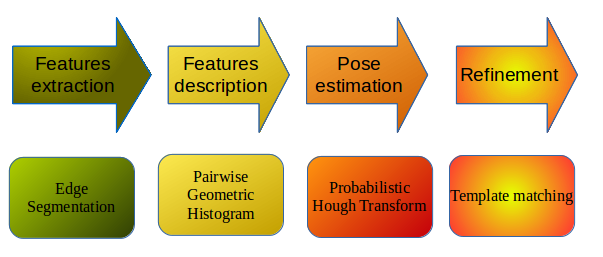
\includegraphics[height=3.5cm]{images/flow_step.png}	
		\end{center}
	\end{itemize}
\end{frame}
\section{Method}
%\subsection{Segmentation}
\begin{frame}{Method - Edge segmentation}
	Purpose: 
	\begin{itemize}
		\item Extract the features (edge) from images
		\item Get the approximate segment lines
	\end{itemize}
	Method:
	\begin{itemize}
		\item Indicate the threshold value by analysis histogram of image		
		\item Canny algorithm
		\item Break edge algorithm$^{\footnote{Thacker, Neil A., P. A. Riocreux, and R. B. Yates. \textit{``Assessing the completeness properties of pairwise geometric histograms."} Image and Vision Computing 13.5 (1995): 423-429.}}$
	\end{itemize}
	Parameters:
	\begin{itemize}
		\item Threshold value: indicated by histogram analysis
		\item Canny ratio: 1:3 (lower:upper)
		\item Minimum distance to stop break edge: 3 pixels
	\end{itemize}
\end{frame}
\begin{frame}{Method - Edge segmentation}
	\begin{columns}[c]
		\column{0.5\textwidth}
		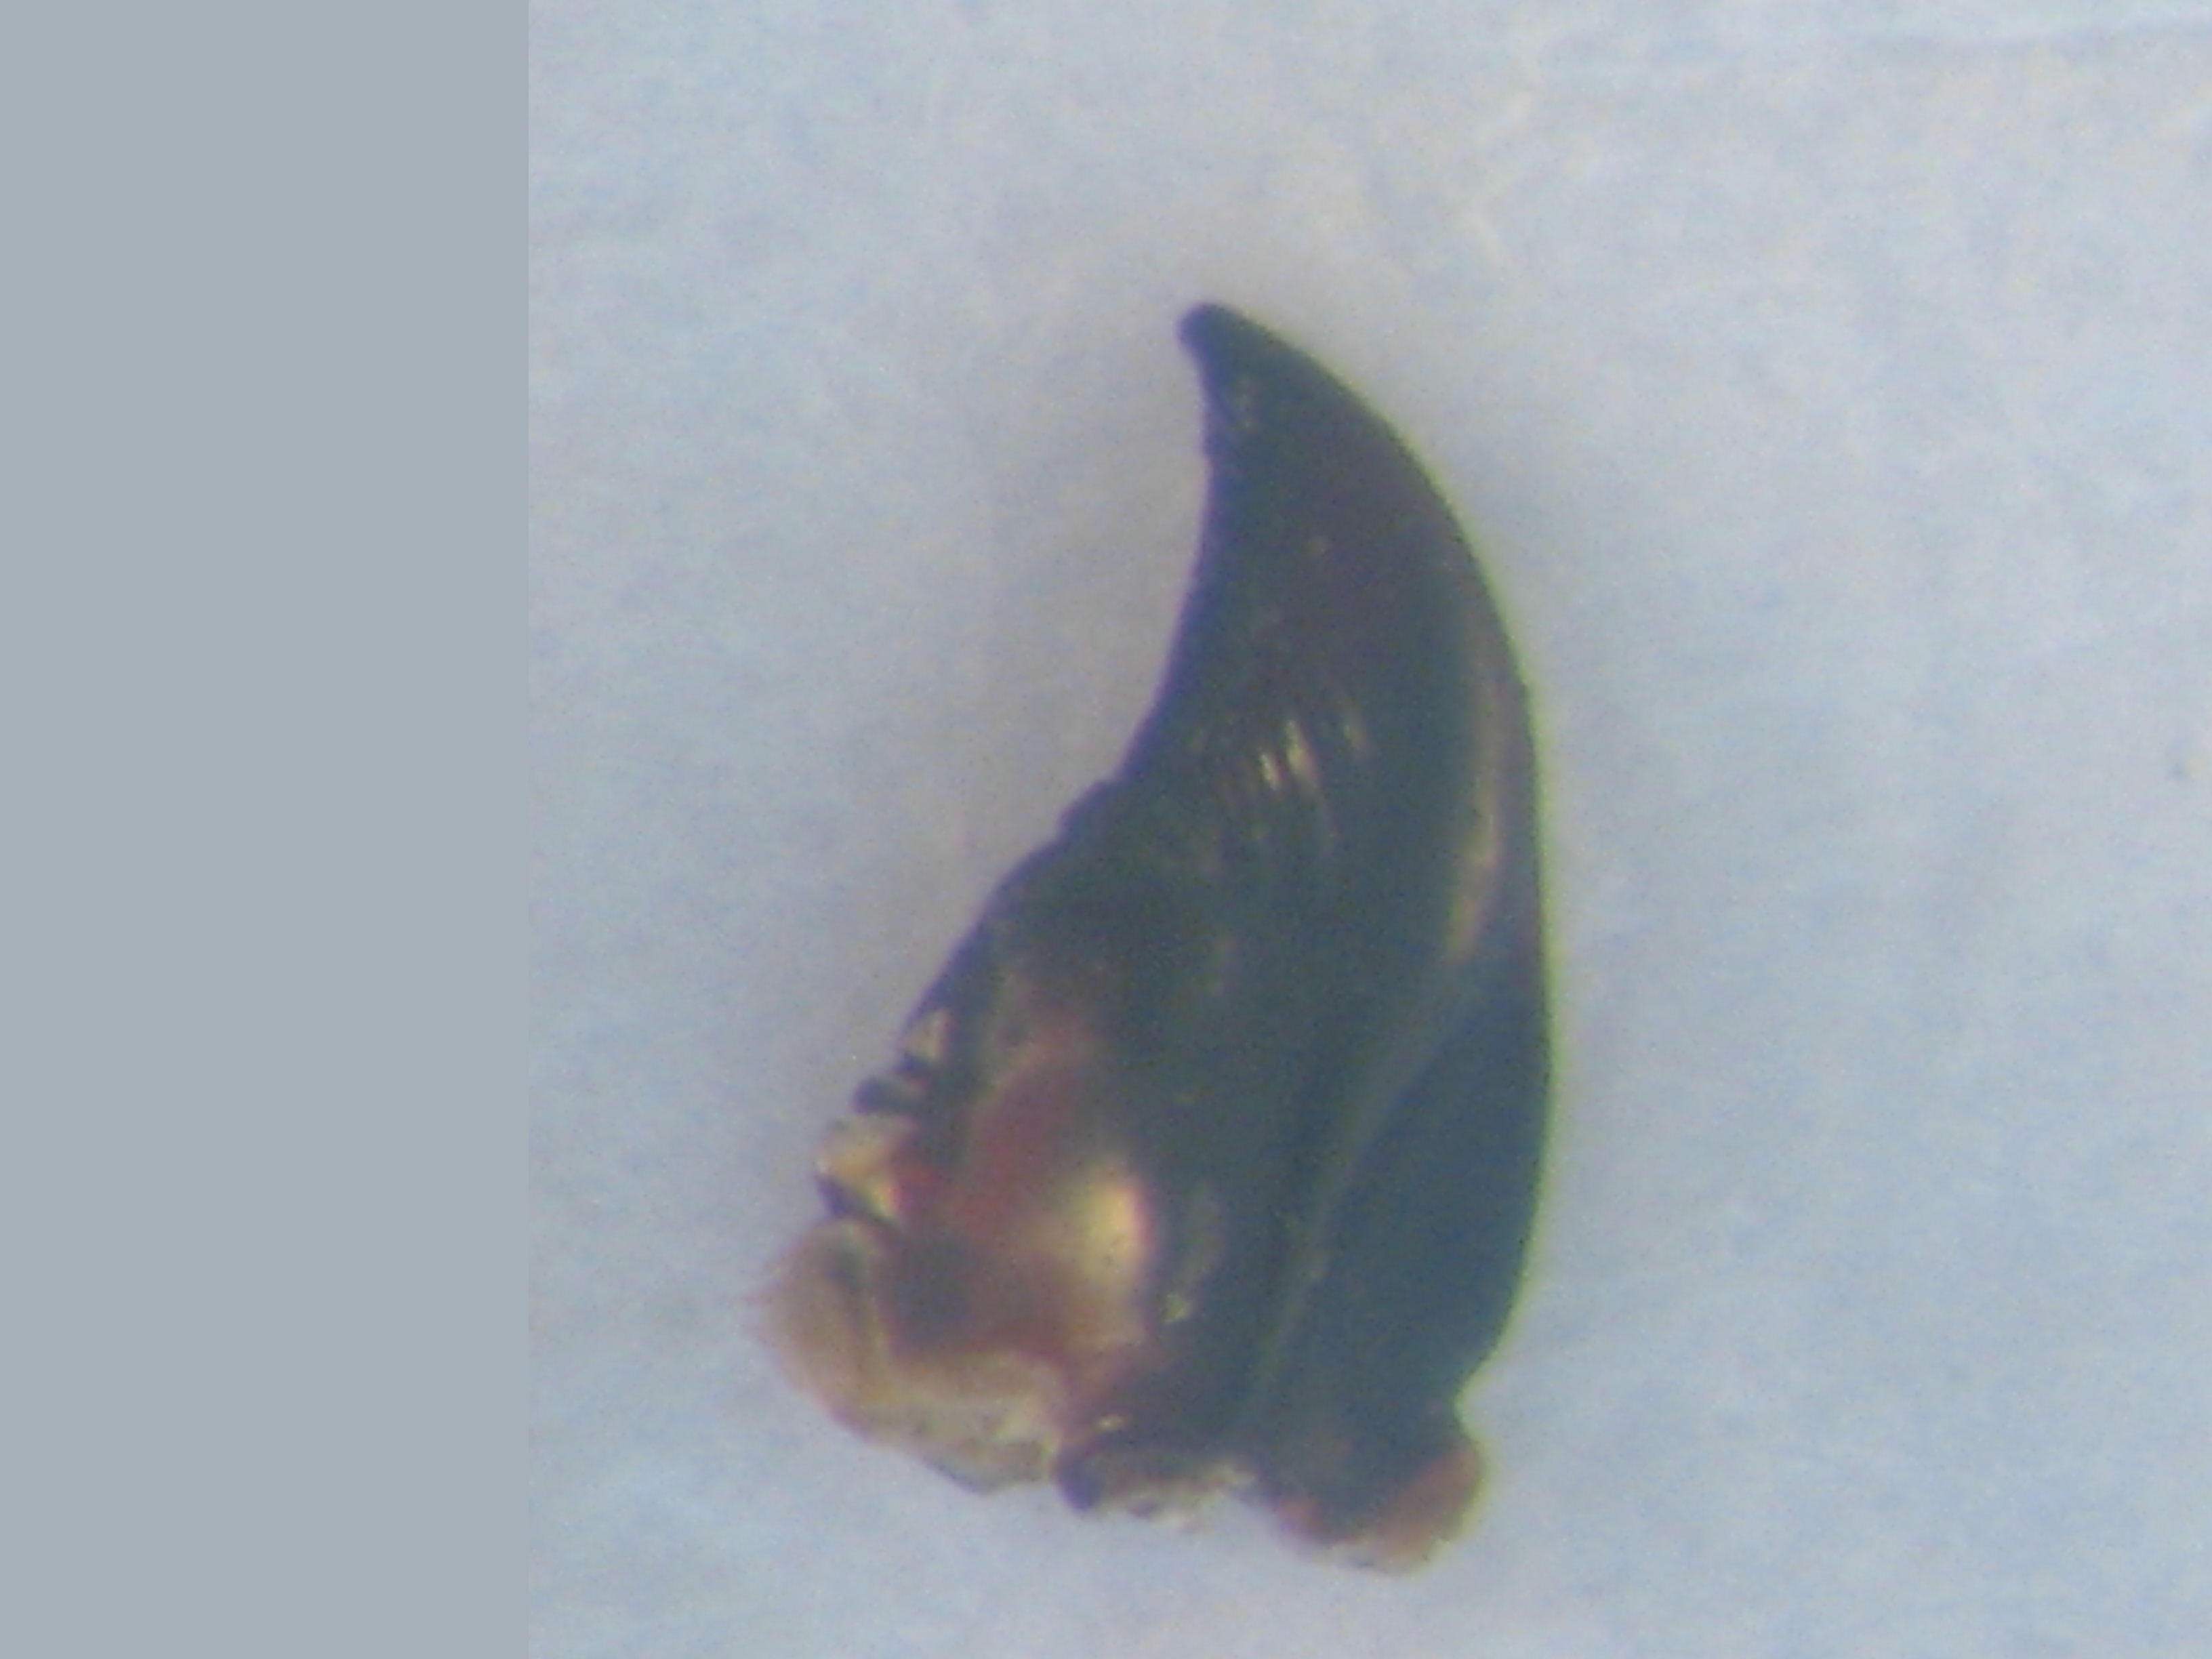
\includegraphics[height=4.5cm]{images/model28.JPG}
		\column{0.5\textwidth}
		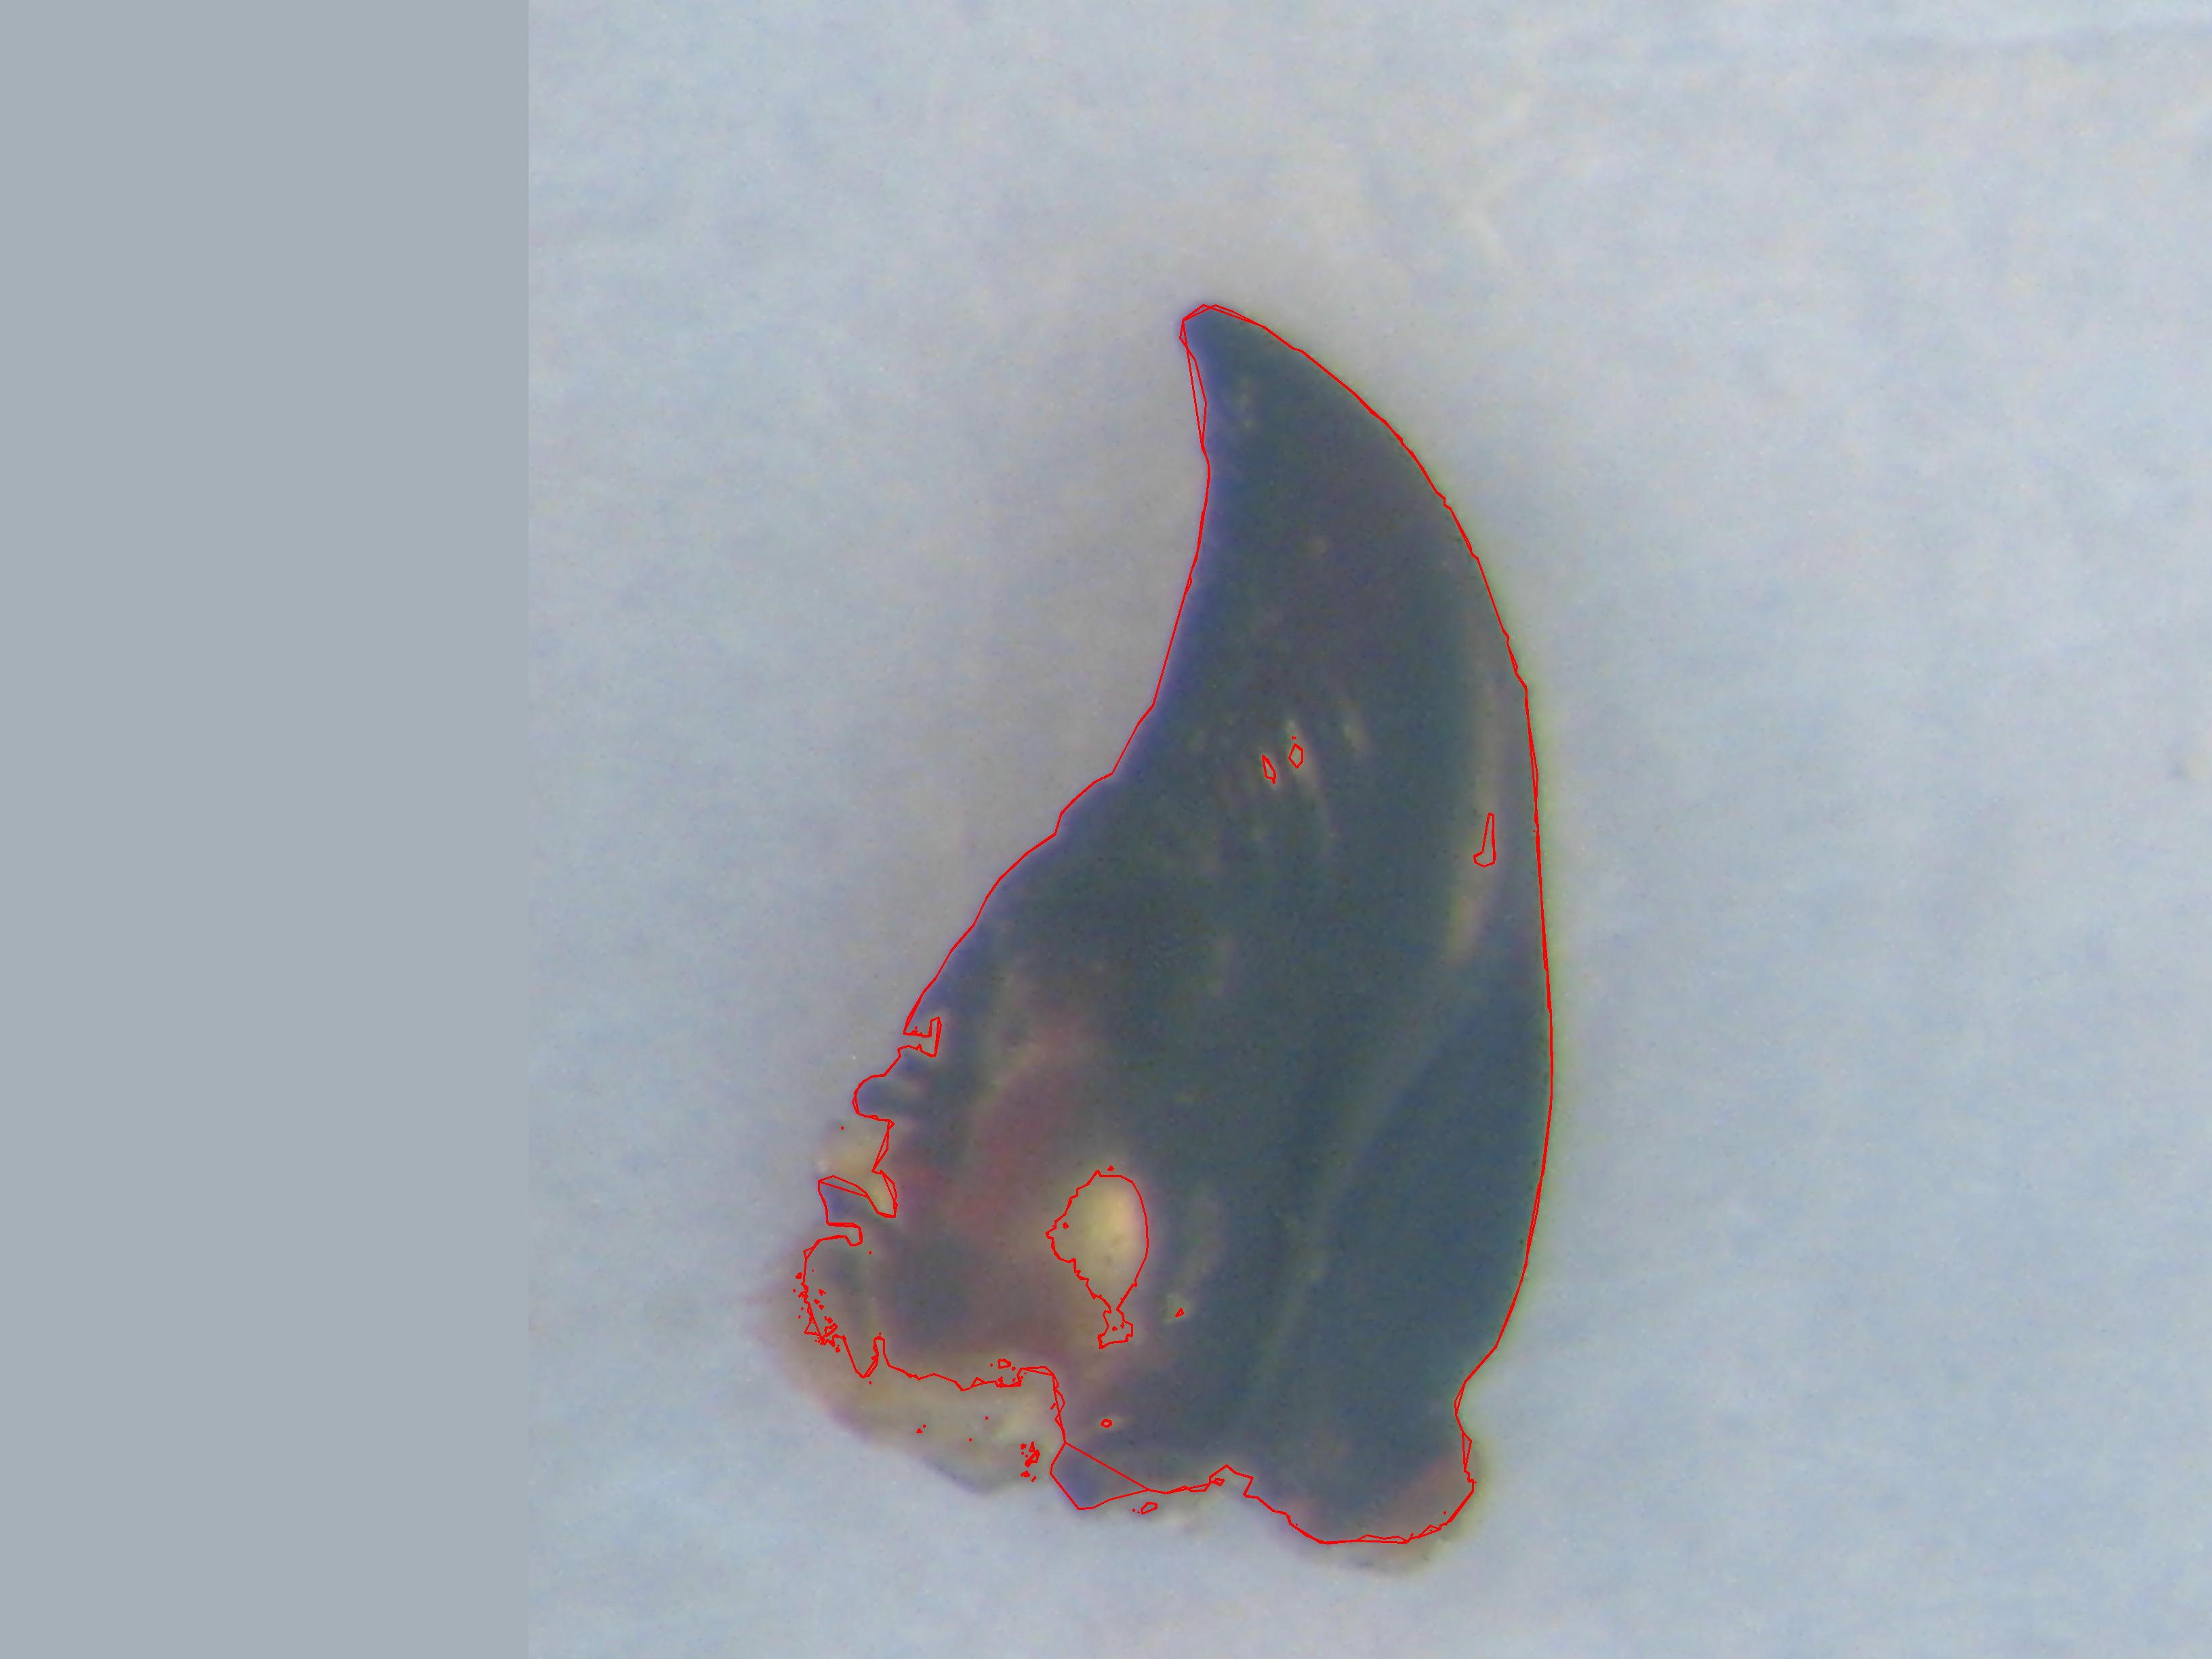
\includegraphics[height=4.5cm]{images/edge28.jpg}
	\end{columns}
\end{frame}
%\subsection{Pairwise geometric histogram(PGH)}
\begin{frame}{Method - Pairwise geometric histogram}
	\begin{description}
		\item[Purpose:] detecting the present of scene image in model image
		\item[Method$^{\footnote{Thacker, Neil A., P. A. Riocreux, and R. B. Yates. \textit{``Assessing the completeness properties of pairwise geometric histograms."} Image and Vision Computing 13.5 (1995): 423-429.}}$:]
		\begin{itemize}
			\item Construct the \textbf{local PGH} for each line
			\item Construct the \textbf{shape PGH}, it is a set of local PGH
			\item Matching shape's PGH by Bhattacharyya metric
		\end{itemize}
		\item[PGH information:] angle between two lines and perpendicular distance from two endpoints of scene line to reference line.
		\item[Parameters]: to build the PGH matrix (used to compute the metric)
			\begin{itemize}
				\item Rows: 90, \textcolor{red}{180}, 360, 720 - presented for angle accuracy
				\item Columns: 250, \textcolor{red}{500}, 1000 - presented for distance accuracy
			\end{itemize}
	\end{description}
\end{frame}
%\subsection{Probabilistic Hough Transform}
\begin{frame}{Method - Probabilistic Hough Transform}
	\begin{description}
		\item[Purpose:]
			\begin{itemize}
				\item Determine the presence and location of model image in scene image
				\item Estimate the landmarks in the scene image
			\end{itemize}
		\item[Method:]
		\begin{itemize}
			\item Build the reference table
			\item Find the pair of scene lines have the best ``vote" with pair of model lines
			\item Estimate the ``reference point" in scene image
			\item Estimate the landmarks
		\end{itemize}
		\item[Result:] Estimated model landmarks on scene image
	\end{description}
\end{frame}
\begin{frame}{Method - PHT parameters (Building the reference table)}
	\texttt{For each \textbf{closet} pair of model lines, compute the perpendicular distance and angle from the line to \textbf{reference point} and save into table}\\[0.3cm]
	\textbf{Reference point}: an arbitrary point in model image (in program, reference point is center point of model image)\\[0.3cm]
	Example:
	\begin{center}
		\begin{tabular}{|c|c|c|}
		\hline
			Pair lines & space 1 & space 2 \\ \hline
			(\textcolor{red}{l1},\textcolor{blue}{l2}) & (\textcolor{red}{30;110.33}) & (\textcolor{blue}{23.5; 855})  \\ \hline
			(\textcolor{red}{l1},\textcolor{green}{l3}) & (\textcolor{red}{15; 121.5}) & (\textcolor{green}{5.5; 200})   \\ \hline
		\end{tabular}
	\end{center}
	Parameters:
	\begin{itemize}
		\item Minimum length of each line: 60 pixels
		\item Minimum angle between two lines: 15 degrees
		\item Distance from an endpoint of a line to another line: 5 pixels
	\end{itemize}
\end{frame}
\begin{frame}{Method - PHT Parameters (Find the best vote of scene)}
	The process to find the best vote are followed:
	\begin{itemize}
		\item \texttt{Create an accumulator}
		\item \texttt{For each \textbf{closet} pair of scene lines, find the pair of model line reasonable agreement about the \textbf{position, orientation and scale}. Get the information about angle and distance}
		\item \texttt{Increase the value in accumulator at relative position}
		\item \texttt{Keep the position where has the maximum value.}
		\item \texttt{Keep the pair of scene line and the entry in reference table}
	\end{itemize}
	Parameters:
	\begin{itemize}
		\item Maximum difference angle: 1 degree
		\item Maximum difference scale: 1 pixel
		\item Maximum difference position: 2 pixels
	\end{itemize}

\end{frame}
\begin{frame}{Method - Probabilistic Hough Transform}
	\begin{center}
		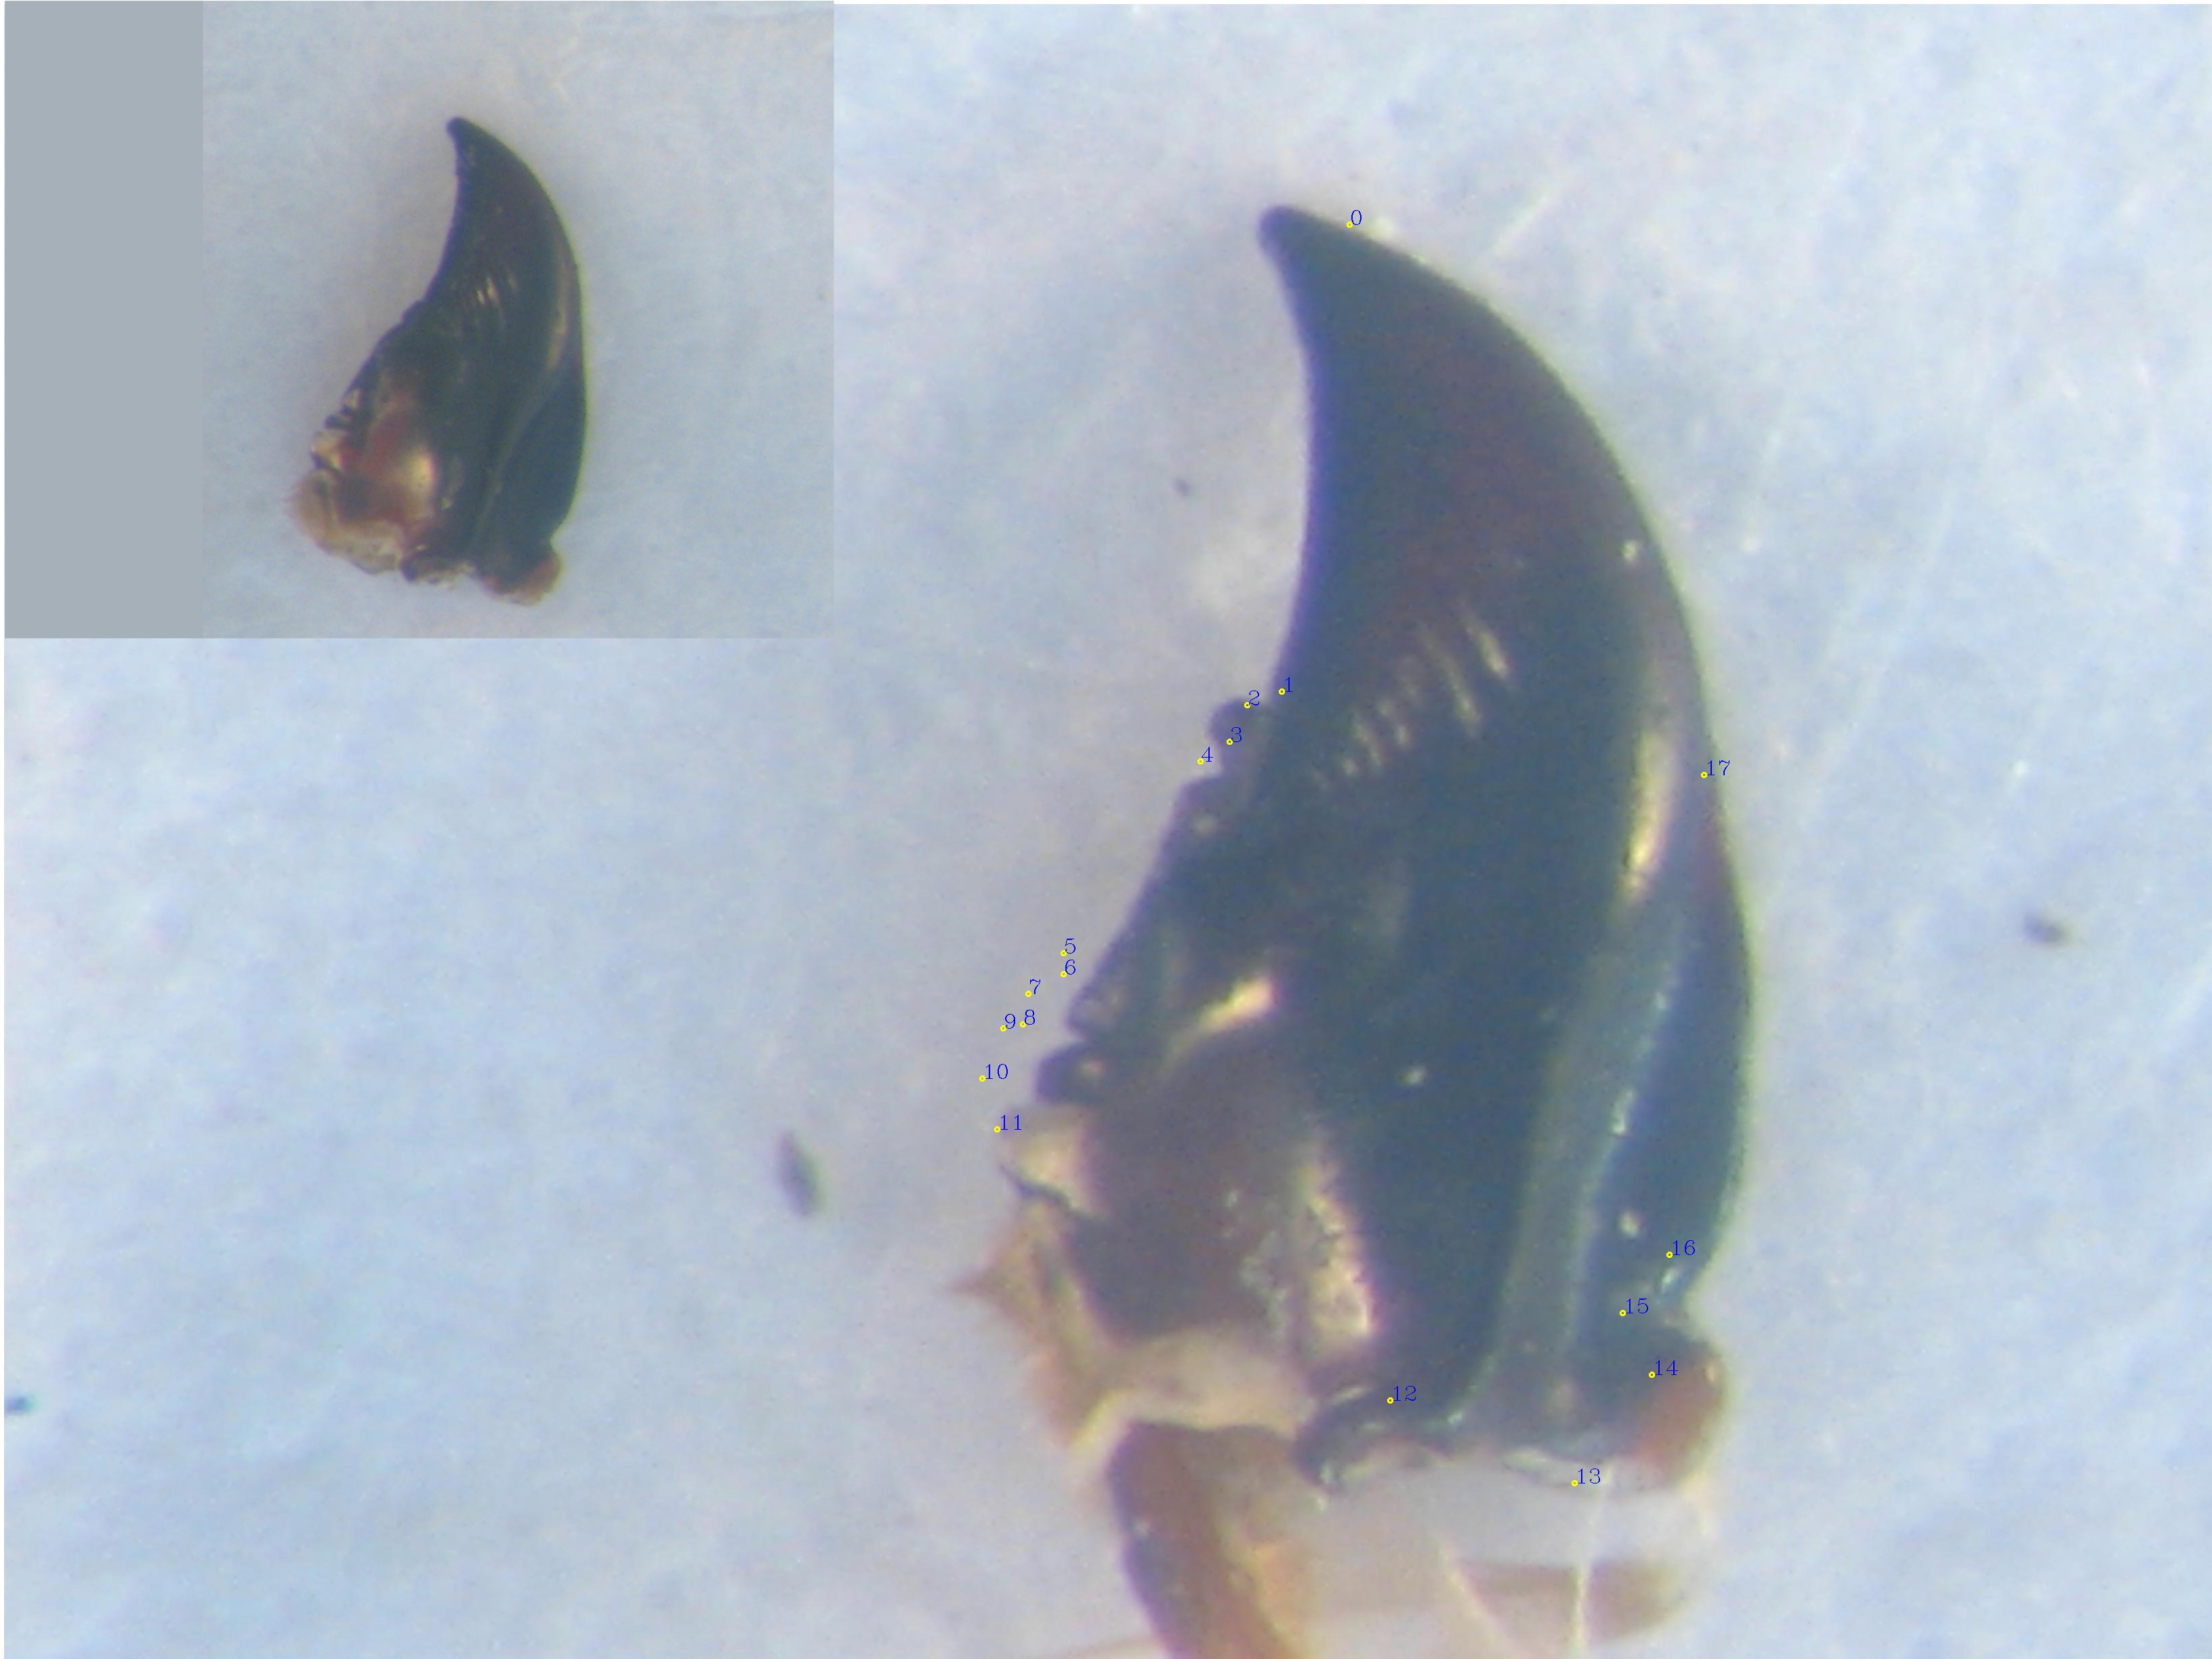
\includegraphics[height=8cm]{images/pht19.JPG}	
	\end{center}
\end{frame}
%\subsection{Template matching}
\begin{frame}{Method - Template matching}
	\begin{description}
		\item [Purpose:] Refine the estimated landmarks on the scene image 
		\item [Method:] 
			\begin{itemize}
				\item On model image: For each landmark, create a bounding box with size ``\textit{t1}" and \textit{landmark} is center point of box
				\item Rotate scene image to match with model
				\item On scene image: For each estimated landmark, create a bounding box with size ``\textit{t2}" and \textit{landmark} is center point of box
				\item Sliding \textit{t1} on \textit{t2} and find the the best match (cross-correlation)
			\end{itemize}
		\item [Parameters:]
			\begin{itemize}
				\item Template box size: 400px (\textbf{EstTemplSize})
				\item Image box size: 1400px (\textbf{EstImageSize})
			\end{itemize}
	\end{description}
\end{frame}
\begin{frame}{Method - Template matching}
	\begin{center}
		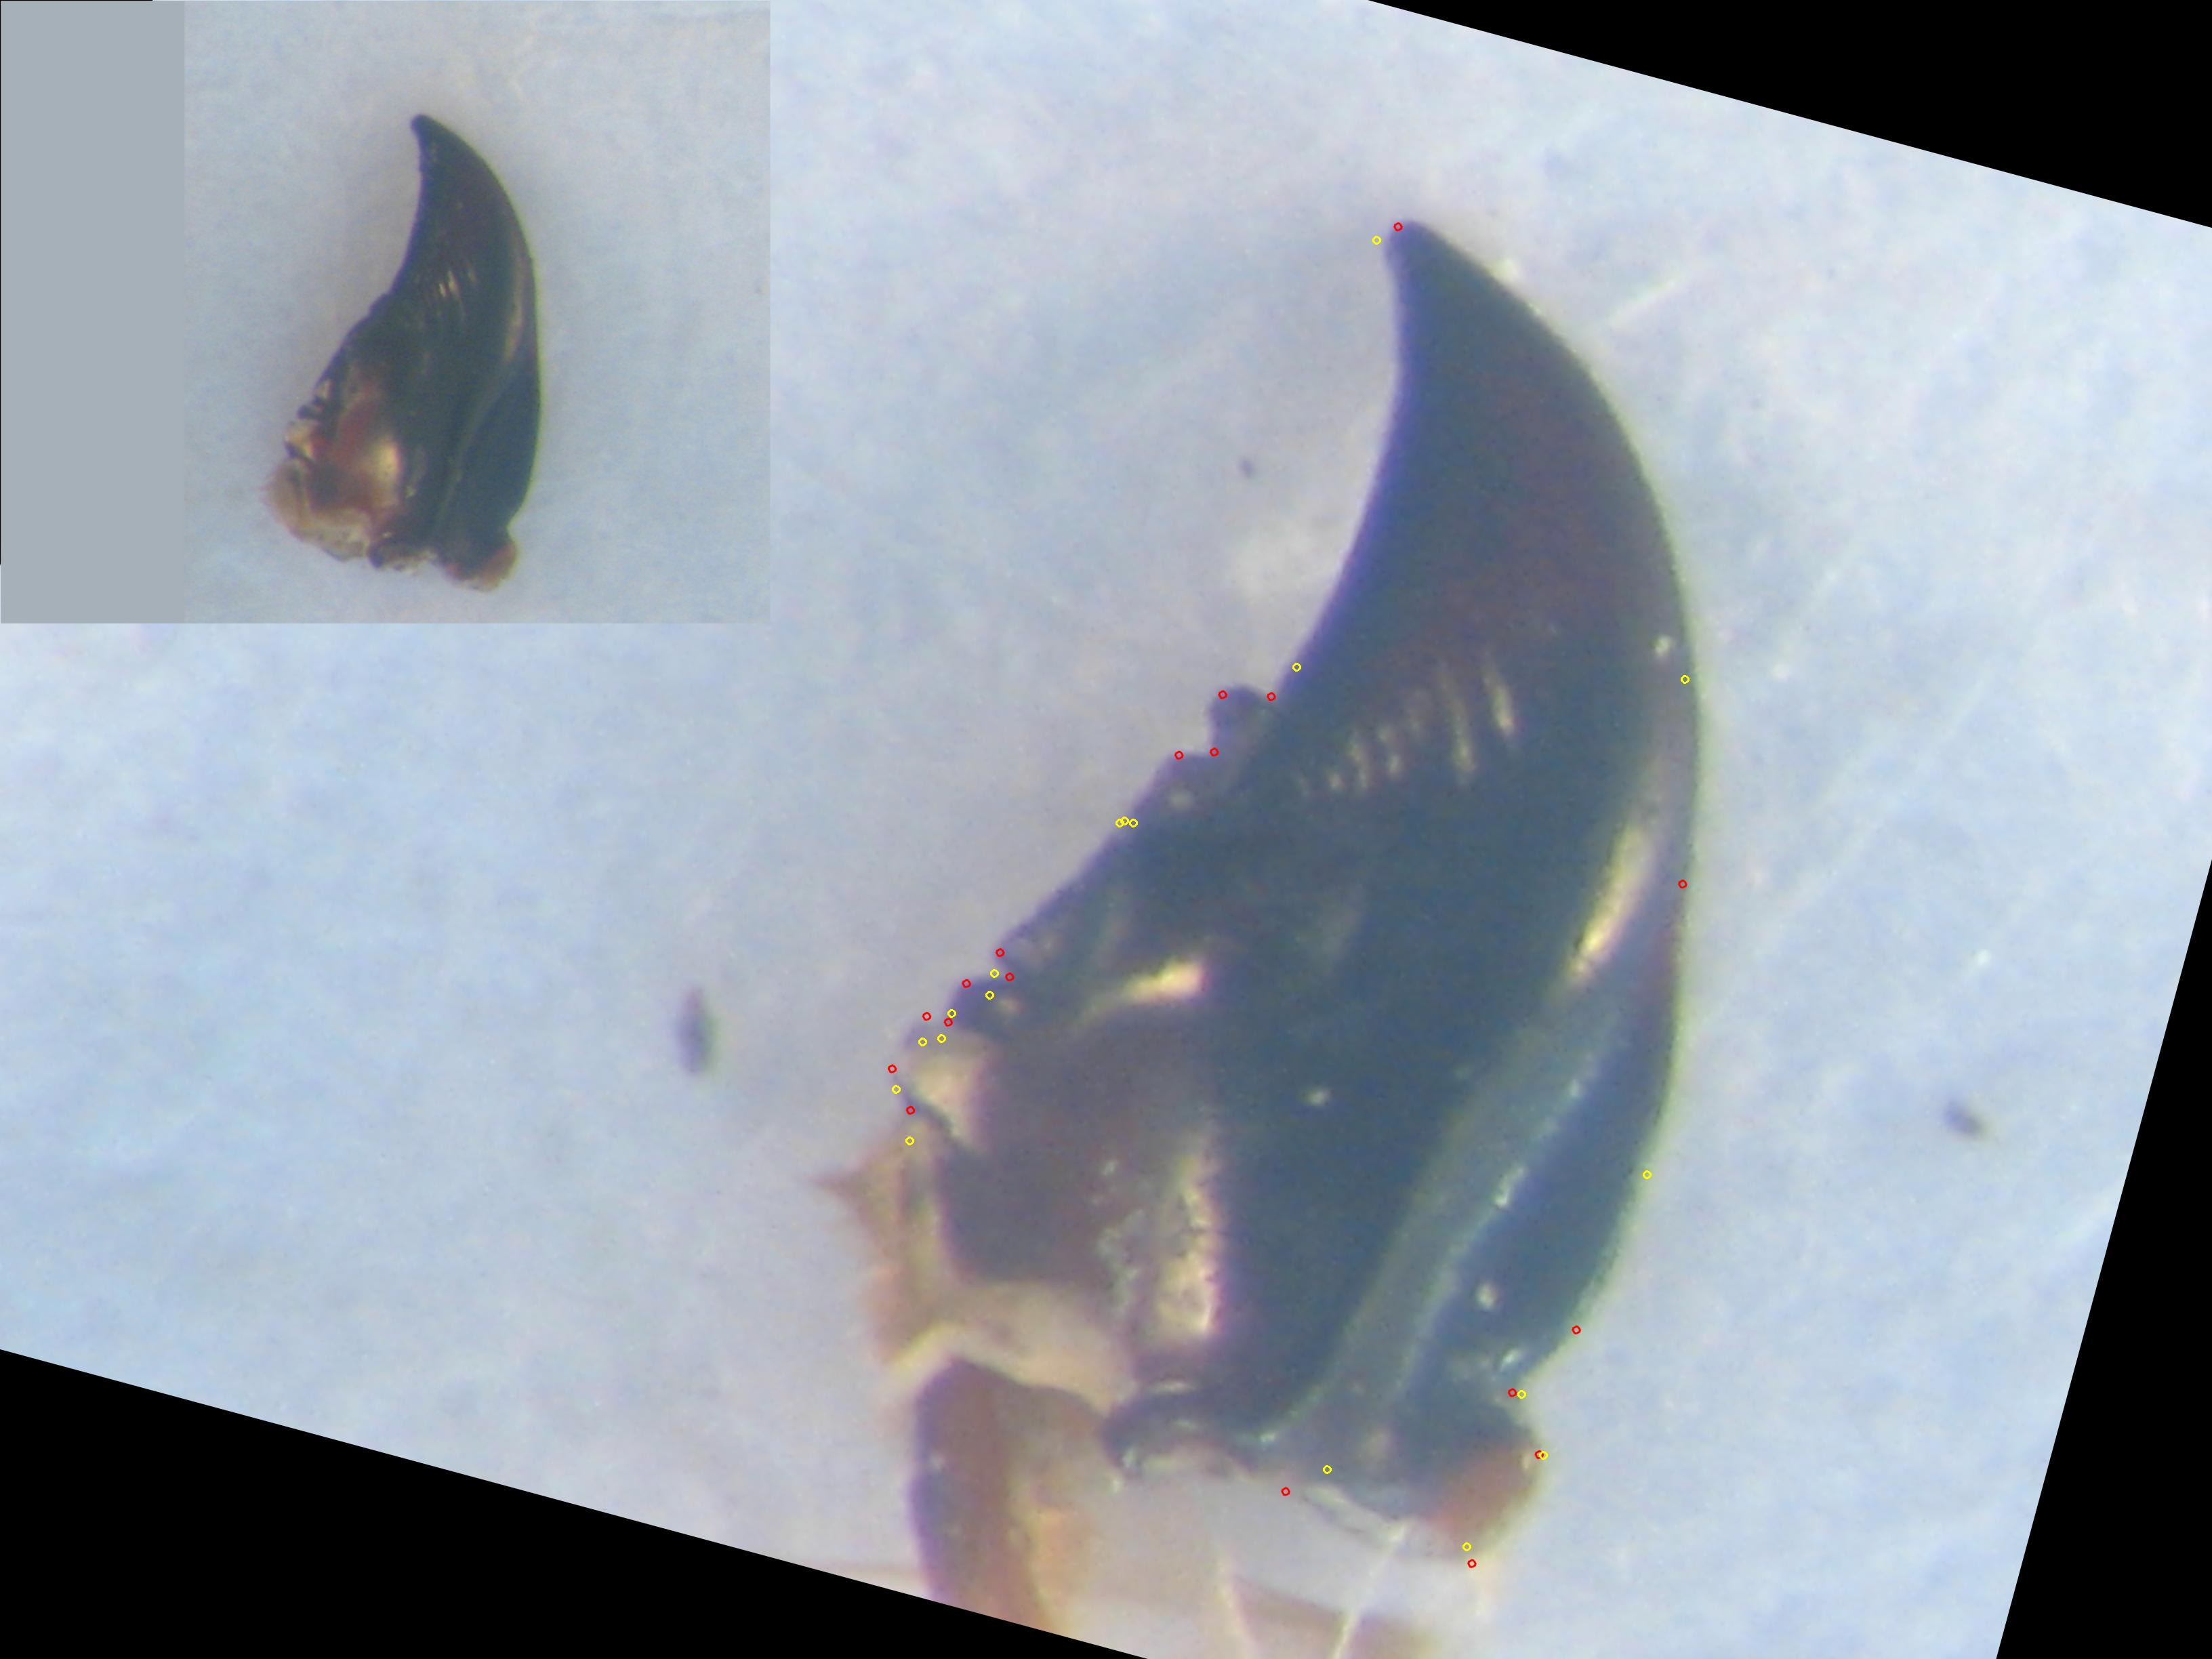
\includegraphics[height=8cm]{images/est19.JPG}	
	\end{center}
\end{frame}
\section{Result}
\begin{frame}Result
	Examination: \\[0.3cm]
	Dataset includes 291 images.
	\begin{enumerate}
		\item Intel(R) Core(TM) 2 Duo CPU T8100 2.1GHz, 2 GB of RAM
			\begin{center}
				\begin{tabular}{|c|c|c|}
					\hline
					No Of images & Segmentation(second) & Estimation(second) \\ \hline
					1 & 0.844 & 31.4245   \\ \hline
					291 & 571.576 & 13000.9131   \\ \hline
				\end{tabular}
			\end{center}
		\item Intel(R) Core(TM) i7-4790 CPU 3.6GHz, 16 GB of RAM.
			\begin{center}
			\begin{tabular}{|c|c|c|}
				\hline
				No Of images & Segmentation(second) & Estimation(second) \\ \hline
				1 & 0.27782 & 10.4392   \\ \hline
				291 & 171.589 & 4665.79   \\ \hline
			\end{tabular}
			\end{center}
	\end{enumerate}
\end{frame}
\begin{frame}{Result}
	\begin{itemize}
		\item Dataset: \textit{Mandibule droite} and \textit{mandibule gauche}
		\item Method includes 4 steps. The result of each step can effect to next step.
		\item This method can be used to identify the landmarks. But, in some cases, the estimated landmarks are not close with manual landmarks.
	\end{itemize}
\end{frame}
\begin{frame}[plain]
  \Huge{\centerline{Thank you !}}
\end{frame}
\end{document}